% intensity
% spectral distribution
% solar geometry
% saules stāvoklis debesīs
% un virziens, kurā stara starojums krīt uz dažādu virzienu un ēnojuma virsmām

\section{Saules diennakts kustība}\label{section:kustiba}

Šajā nodaļā Saules apstarojums tiek aplūkots no ģeometriskajiem apsvērumiem - virziena, no kura staru kūlis sasniedz virsmu, leņķi uz virsmas un gada gaitā saņemtā starojuma daudzuma.

Ģeometriskās sakarības starp saules paneļa virsmas plakni un ienākošo Saules starojuma kūli jeb Saules pozīcija relatīvi pret šo plakni tiek aprakstīta ar vairākiem leņķiem. Ar $\theta$ apzīmēsim staru krišanas leņķi uz saules paneli, pieņemot saules paneli par nekustīgu plakni. Tad, pie nemainīgas starojuma intensitātes, paneļa saņemtā enerģija būs proporcionāla $\cos{\theta}$ (ja $\theta<90^\circ$) vai būs vienāda ar 0 (ja $\theta \geq 90^\circ$, t.i., Saules stari krīt uz paneļa apakšējo virsmu) pēc formulas \ref{eq:apgaismojums}. Saules diennakts kustība, gadalaiku cikls, kā arī saules paneļa novietojums ir ievēroti $\cos{\theta}$ aprēķina izteiksmē \ref{eq:theta}, kur lietotie leņķi definēti \ref{tab:theta} tabulā~\cite{ThermalProcesses}.

\begin{equation}
\label{eq:apgaismojums}
E = I \cdot cos(\theta)
\end{equation}
\begin{equation}
\label{eq:theta}
\begin{aligned}
\cos{\theta} = {} & \sin{\delta} \sin{\phi} \cos{\beta} - \sin{\delta} \cos{\phi} \sin{\beta} \cos{\gamma} +                           \\
	& \cos{\delta} \cos{\phi} \cos{\beta} \cos{\omega} + \cos{\delta} \sin{\phi} \sin{\beta} \cos{\gamma} \cos{\omega} + \\
	& \cos{\delta} \sin{\beta} \sin{\gamma} \sin{\omega},
\end{aligned}
\end{equation}

Saules deklināciju solārajā pusdienlaikā var aprēķināt pēc lietderīgas aproksimācijas, kur $n$ apzīmē dienas kārtas numuru gadā. \cite{cooper1969}.
\begin{equation}
\label{eq:delta}
    \delta = 23 \sin \left( 360 \cdot \frac{284+n}{365} \right),
\end{equation}

Ar vienādojumu \ref{eq:theta} un \ref{eq:delta} palīdzību ir iespējams aprēķināt $\cos{\theta}$ laika atkarību, kas ir pirmais tuvinājums Saules apstarojuma izmaiņām dienas laikā.
Parametru vērtības katram no darbā lietotajiem Saules paneļiem ir apkopotas \ref{tab:param}. tabulā.
Lietojot šos parametrus, tika aprēķināta $\cos{\theta}$ atkarība no laika diviem datumiem: 1. janvārim un 30. aprīlim (skat. \ref{fig:cos-theta}. att.). No tā secināms, ka austrumu virzienā uzstādītais panelis saņem vairāk apstarojuma no rīta nekā rietumu virzienā vērstais panelis. Pēc šī aprēķina iespējams prognozēt paneļu saražotās enerģijas izmaiņas gada griezumā, piemēram, no dienvidu paneļiem janvārī efektīvākais ir 90$^\circ$ leņķī vērstais, jo Saule atrodas zemu pie horizonta, bet aprīlī efektīvākais ir 40$^\circ$ leņķī.

\begin{table}[h!]
\caption{Leņķu, kas lietoti \ref{eq:theta} vienādojumā, definīcijas.}
\begin{center}
\begin{tabular}{|c|c|l|}\hline
	         &         Apgabals         & Definīcija\\ \hline
	$\theta$ &  $(0^\circ;180^\circ)$   & staru krišanas leņķis uz Saules paneli\\ \hline
	$\delta$ &  $(-23^\circ;23^\circ)$  & Saules deklinācija\\ \hline
	 $\phi$  &  $(-90^\circ;90^\circ)$  & ģeogrāfiskais platums\\ \hline
	$\beta$  &  $(0^\circ;180^\circ)$   & paneļa slīpums \\ \hline
	$\gamma$ & $(-180^\circ;180^\circ)$ & paneļa azimuts \\ \hline
	$\omega$ & $(-180^\circ;180^\circ)$ & solārais stundu leņķis\\ \hline
\end{tabular}
\end{center}
\label{tab:theta}
\end{table}

\begin{table}[h!]
	\caption{Darbā lietotajiem Saules paneļiem atbilstošās leņķisko parametru vērtības, grādos.}
	\begin{center}
		\begin{tabular}{|r|c|c|c|c|c|}
			\hline
			         & R.13 & A.13 &   D.13   & D.40 & D.90 \\ \hline
			paneļa slīpums $\beta$  & \multicolumn{3}{c|}{13} &  40  &  90  \\ \hline
			paneļa azimuts $\gamma$ &  90  & -90  & \multicolumn{3}{c|}{0}  \\ \hline
			ģeogrāfiskais platums $\phi$  &        \multicolumn{5}{c|}{57}        \\ \hline
		\end{tabular}
	\end{center}
	\label{tab:param}
\end{table}

\begin{figure}[h]
	\centering
	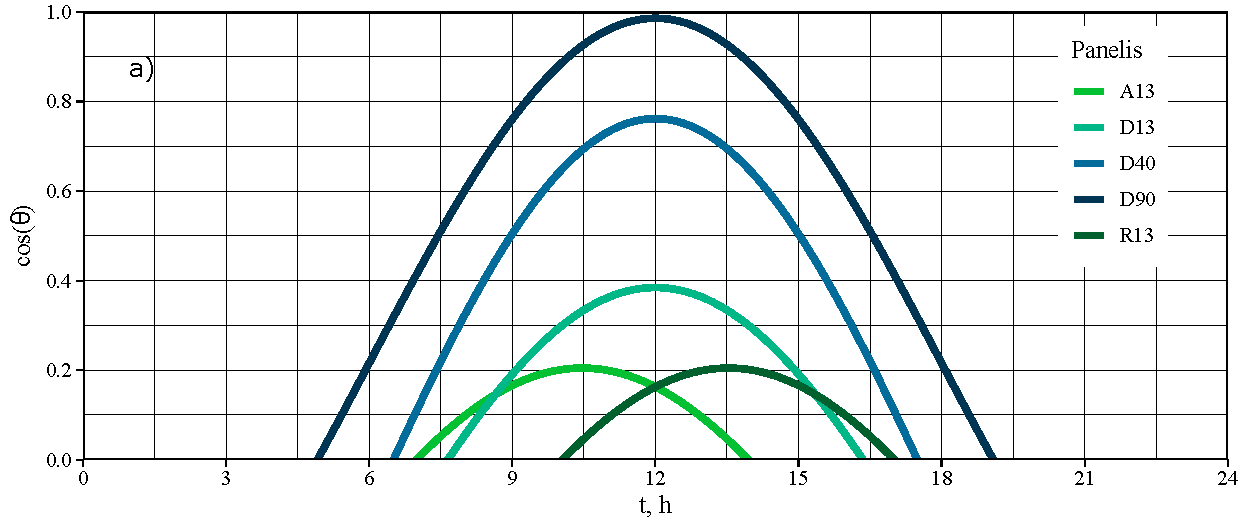
\includegraphics[width=\linewidth]{figures/meteo/jan.pdf}
	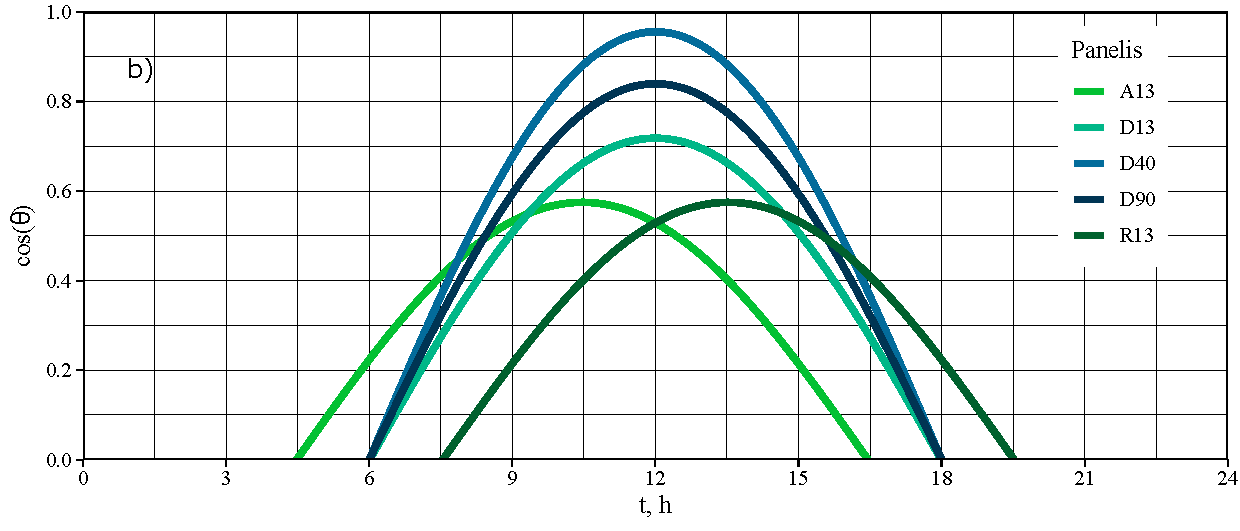
\includegraphics[width=\linewidth]{figures/meteo/mar.pdf}
	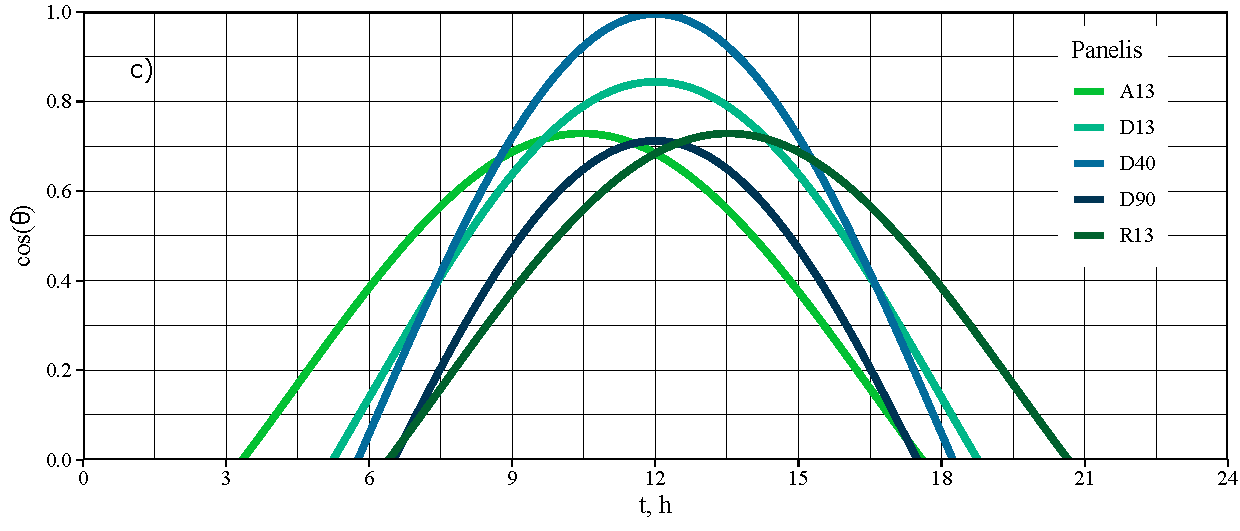
\includegraphics[width=\linewidth]{figures/meteo/apr.pdf}
	\caption{Diennakts laikā paredzētas $\cos(\theta)$ vērtības darbā lietotajiem Saules paneļiem, aprēķinātas pēc \ref{eq:theta} izteiksmes 1. janvārim (a), 1. martam (b), 30. aprīlim (c).}
	\label{fig:cos-theta}
\end{figure}